% First-page letterhead: logo and rule are vector crops of page 2 of
% Heya-Letterhead.pdf (612x792pt; viewports in PDF coordinates):
%   logo ink box  x 72.5-135.4, y(top) 72.5-92.6  -> viewport 71 698 137 721
%   rule          x 70.6-541.4, y(top) ~112.8     -> viewport 70 677 542 682
% The logo sits at the left margin with its top 36pt from the page top;
% the rule spans the text width at 75pt. The date is typeset (not
% cropped) so it can be updated here: a FIXED string, deliberately not
% \today - the CI reproduce-gate compares the committed PDF's words
% against a rebuild, so the date must not depend on the build day. It is
% styled to the template's date (sans, gray 0.42), right-aligned at the
% right margin on the logo's vertical center. Page-one content starts
% just below the rule (25pt clearance minus a 0.9cm tightening).
\usepackage{eso-pic}
\makeatletter
\@ifpackageloaded{xcolor}{}{\usepackage{xcolor}}
\@ifpackageloaded{graphicx}{}{\usepackage{graphicx}}
\makeatother
% Heya-Letterhead-flat.pdf is the template with its text objects stripped
% (gs -dFILTERTEXT): viewport clipping hides but does not remove the
% template page's placeholder text ("Paper Title Goes Here", authors,
% dates), which would otherwise leak into the built PDF's extractable
% text layer (copy-paste, indexing, screen readers). The logo wordmark
% is vector outlines, so it survives the filter untouched.
% Set this to the paper's actual submission/draft date when you start a
% new paper from this template.
\newcommand{\letterheaddate}{2026-07-23}
\AddToShipoutPictureBG*{%
  \put(\LenToUnit{71pt},\LenToUnit{733pt}){%
    \includegraphics[page=2,viewport=71 698 137 721,clip]{Heya-Letterhead-flat.pdf}}%
  \put(\LenToUnit{540pt},\LenToUnit{741.5pt}){%
    \makebox[0pt][r]{\sffamily\fontsize{10}{12}\selectfont
      \textcolor[gray]{0.42}{\letterheaddate}}}%
  \put(\LenToUnit{70pt},\LenToUnit{715pt}){%
    \includegraphics[page=2,viewport=70 677 542 682,clip]{Heya-Letterhead-flat.pdf}}%
}
\AtBeginDocument{\vspace*{\dimexpr 25pt - 0.9cm\relax}}
% Every-page footer: the page number stays centered (as under the
% default plain style) and heya.au sits at the left margin as a live
% link, so the publisher is findable directly from any page rather
% than via the affiliation line. Styled to match the letterhead date
% (sans, gray 0.42) at \footnotesize: small but legible. The inner
% \textcolor deliberately overrides hyperref's colorlinks urlcolor.
\usepackage{fancyhdr}
\pagestyle{fancy}
\fancyhf{}
\renewcommand{\headrulewidth}{0pt}
\fancyfoot[C]{\thepage}
\fancyfoot[L]{\href{https://heya.au}{\sffamily\footnotesize
  \textcolor[gray]{0.42}{heya.au}}}
